\chapter{Análisis de Contexto}

\section{Conjuntos de Datos}
\label{chapter:datasets}
En el ámbito de los algoritmos de superresolución, la elección del conjunto de datos puede influir significativamente en el entrenamiento del algoritmo y, en última instancia, en su rendimiento. Tres conjuntos de datos clave en este dominio son el OpenImage Dataset, el WorldStrat Dataset y el Sen2Venus Dataset. Al contrastar estos conjuntos de datos, es evidente que existen varios compromisos a considerar. Estos compromisos, según la naturaleza de las tareas de superresolución a realizar, podrían influir de manera considerable en la elección del conjunto de datos. El OpenImage Dataset, por ejemplo, destaca por sus pares de imágenes de alta resolución (HR) que alcanzan hasta 0.5 metros. Sin embargo, sus pares de baja resolución (LR) se generan de manera sintética y están geográficamente limitados a los Estados Unidos. En consecuencia, su aplicabilidad global puede ser limitada, lo cual podría restringir su utilidad en escenarios a nivel mundial. El WorldStrat dataset, por otro lado, se destaca por su diversidad, ofreciendo una amplia gama de escenas y paisajes. Esta muestra diversa puede mejorar la capacidad de generalización de los algoritmos de SR. Sin embargo, su enfoque de no filtrar revisitas de baja resolución según la cobertura de nubes introduce una capa adicional de complejidad. Además, es bastante pequeño en comparación con el tamaño de los modelos. Finalmente, el Sen2Venus Dataset es conocido por su buen preprocesamiento que asegura una buena correspondencia entre imágenes de LR y HR en el dominio espectral. Sin embargo, la imagen de alta resolución solo tiene el doble de resolución espacial que la de baja resolución y puede carecer de la diversidad que se encuentra en el WorldStrat dataset. A continuación, se proporciona una explicación más detallada de cada conjunto de datos.

\subsection{OpenImages}
OpenImages es un conjunto de datos popular en visión por computadora que proporciona una gran colección de imágenes etiquetadas para el entrenamiento y evaluación de modelos de aprendizaje automático. El conjunto de datos cubre una amplia gama de conceptos visuales y objetos, incluidos personas, autos, casas, trenes, animales, etc. Se utiliza ampliamente en tareas como la detección de objetos, clasificación de imágenes y detección de relaciones visuales. Para fines de SR, la cantidad y calidad de las anotaciones no son relevantes, sino que es un conjunto de datos de fácil acceso y disponible gratuitamente (CC-BY) que contiene más de millones de imágenes. Los autores originales del modelo de latente-difusión utilizaron este conjunto de datos para entrenar sus puntos de control.

Dado que es un conjunto de datos de visión por computadora, solo contiene imágenes RGB de escenas cotidianas tomadas con cámaras digitales estándar. Por lo tanto, no solo los objetos representados en las imágenes están completamente desvinculados del dominio de la teledetección, sino que sus características espectrales también son muy diferentes. Para entrenar modelos de 4 bandas, se crea artificialmente una cuarta banda a partir de la intensidad de la imagen y se añade en la dimensión de bandas. La imagen de LR se crea interpolando la versión HR al tamaño deseado de 128x128 píxeles.

Los datos en cuestión no están directamente relacionados con el problema de investigación en términos de sus características espectrales, espaciales o de dominio. Sin embargo, el gran volumen de imágenes resulta valioso para entrenar un modelo recién inicializado en atributos y conexiones de imagen fundamentales. Sorprendentemente, al aplicar técnicas de superresolución a imágenes de teledetección utilizando autoencoders y U-Nets de denoising entrenados en el conjunto de datos OpenImages, se han logrado resultados notablemente buenos. Esto demuestra que el conocimiento adquirido a través del entrenamiento en el conjunto de datos OpenImages puede transferirse al dominio de la teledetección y crear una base sólida para el ajuste fino en conjuntos de datos más sofisticados.

\begin{figure}[H] 
    \caption{\doublespacing \\ \textit{Ejemplo de un par de imágenes LR y HR de OpenImages.}} 
    \centering
    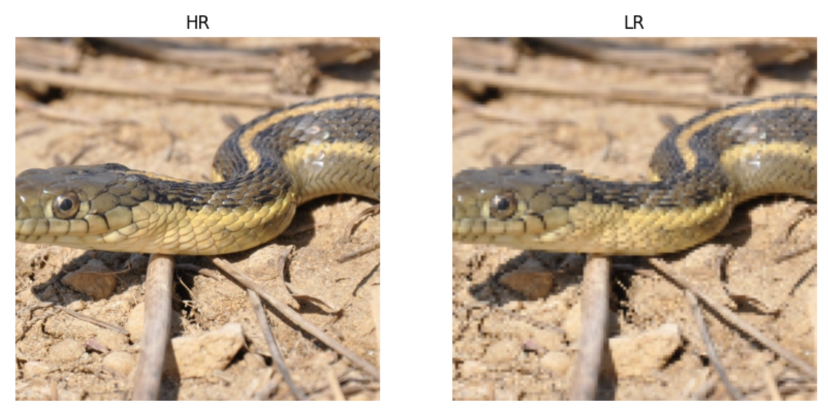
\includegraphics[width=1\linewidth]{images/openimages_example.png}
    \begin{justify}
        \textit{Nota.} Ejemplo de un par de imágenes LR y HR de OpenImages.
    \end{justify}                    
    \label{fig:openimages_example}
\end{figure}

\subsection{Sentinel-2 Dataset}

\subsection{NAIP Dataset}
El Programa Nacional de Imágenes de Agricultura (NAIP) adquiere imágenes aéreas de alta resolución de áreas agrícolas en los Estados Unidos. Proporciona imágenes actuales y precisas para apoyar aplicaciones agrícolas y la toma de decisiones. NAIP captura imágenes con una resolución espacial de 0.6 metros, lo que permite un análisis detallado de las actividades agrícolas. Utilizando plataformas aéreas especializadas con sensores multiespectrales, NAIP recopila datos en varias bandas espectrales, incluyendo rojo, verde, azul e infrarrojo cercano. El conjunto de datos NAIP cubre diversas regiones agrícolas y se actualiza regularmente. Está disponible al público de forma gratuita, facilitando su uso en investigación agrícola, agricultura de precisión, gestión de tierras y aplicaciones relacionadas. Se muestra una comparación entre Sentinel-2 y NAIP en la Figura \ref{fig:naip_comparison}.

\begin{figure}[H] 
    \caption{\doublespacing \\ \textit{Comparación entre Sentinel-2 y NAIP cerca de Rapid City, Dakota del Sur.}} 
    \centering
    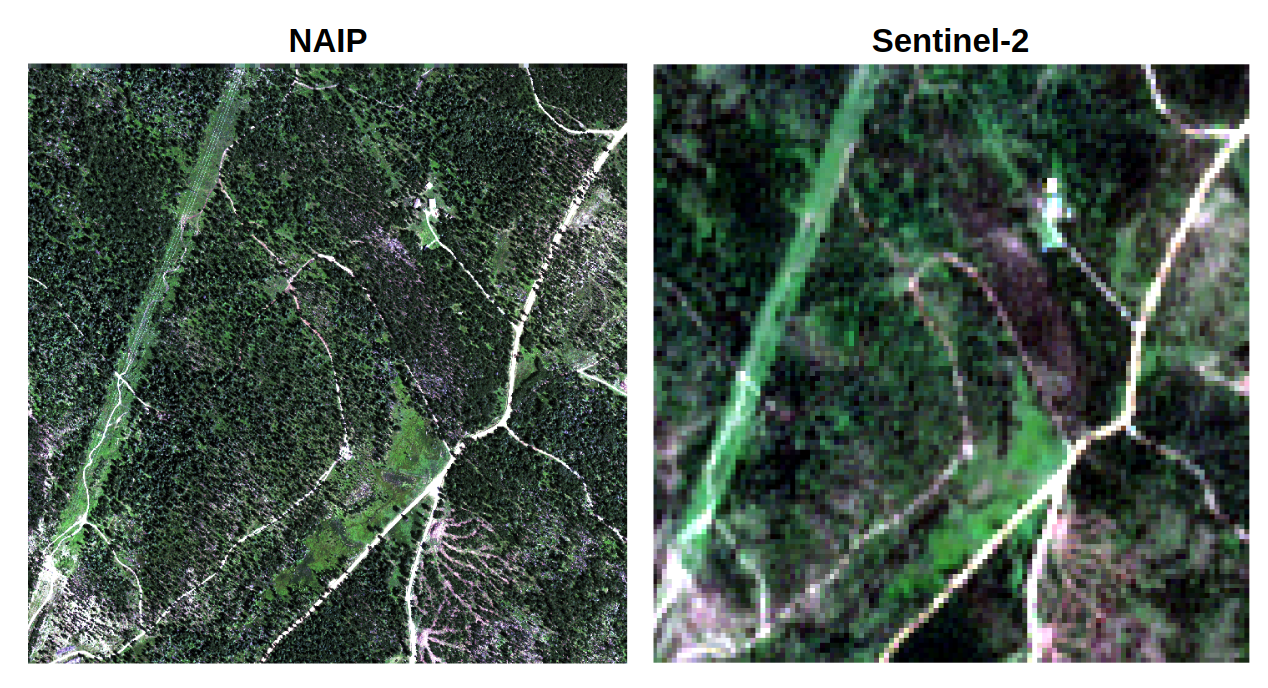
\includegraphics[width=1\linewidth]{images/csaybar_fig02.png}
    \begin{justify}
        \textit{Nota.} Comparación entre Sentinel-2 y NAIP cerca de Rapid City, Dakota del Sur. La imagen de Sentinel-2 (derecha) tiene una resolución espacial de 10 metros, mientras que la imagen de NAIP (izquierda) tiene una resolución espacial de 0.6 metros.
    \end{justify}                    
    \label{fig:naip_comparison}
\end{figure}

\subsection{OpenSR dataset}
El conjunto de datos OpenSR es un conjunto de datos extenso diseñado para facilitar el desarrollo de algoritmos estándar y de referencia para superresolución de imágenes individuales de Sentinel-2. Las imágenes de alta resolución (HR) en este conjunto de datos provienen del Programa Nacional de Imágenes de Agricultura (NAIP), que proporciona imágenes aéreas que cubren todo el territorio continental de los Estados Unidos.

NAIP recopila datos en varias bandas espectrales, incluyendo rojo, verde, azul e infrarrojo cercano, con una resolución de 0.6 m/píxel.

\subsection{WorldStrat Dataset}
El Conjunto de Datos Estratificados Mundial, conocido también como WorldStrat, es un conjunto de datos diverso y curado. Su objetivo principal es apoyar el desarrollo de algoritmos de superresolución multiframe diseñados específicamente para imágenes Sentinel-2. Una característica clave de este conjunto de datos es la inclusión de imágenes de alta resolución (HR) obtenidas de los satélites SPOT 6/7. Las imágenes de SPOT abarcan cinco bandas espectrales distintas. La banda pancromática (PAN) tiene una resolución de 1.5 m/píxel y las bandas restantes, incluyendo Rojo, Verde, Azul e Infrarrojo Cercano (RGBNIR), tienen una resolución de 6 m/píxel.

El conjunto de datos abarca aproximadamente 10,000 kilómetros cuadrados e incluye 3,504 áreas de interés distintas (Figura \ref{fig:worldstrat}), seleccionadas para maximizar la diversidad de usos posibles. El presupuesto de adquisición de imágenes para el conjunto de datos se divide en tres partes:

\begin{itemize}
    \item \textbf{Asentamientos/Urbanos:} Esta parte cubre 3,647.5 kilómetros cuadrados con 1,459 imágenes de alta resolución. Las imágenes son una muestra estratificada basada en la densidad urbana (SMOD).
    \item \textbf{No-Asentamientos}: Esta parte cubre 2,370 kilómetros cuadrados con 948 imágenes de alta resolución. Las imágenes son una muestra estratificada basada en el uso del suelo (IPCC).
    \item \textbf{Subrepresentados}: Esta parte cubre 3,802.5 kilómetros cuadrados con 1,521 imágenes de alta resolución. Las fuentes de estas imágenes incluyen UNHCR, Amnistía y ASMSpotter.
\end{itemize}

\begin{figure}[H] 
    \caption{\doublespacing \\ \textit{Resumen de la construcción y clases del conjunto de datos WorldStrat.}} 
    \centering
    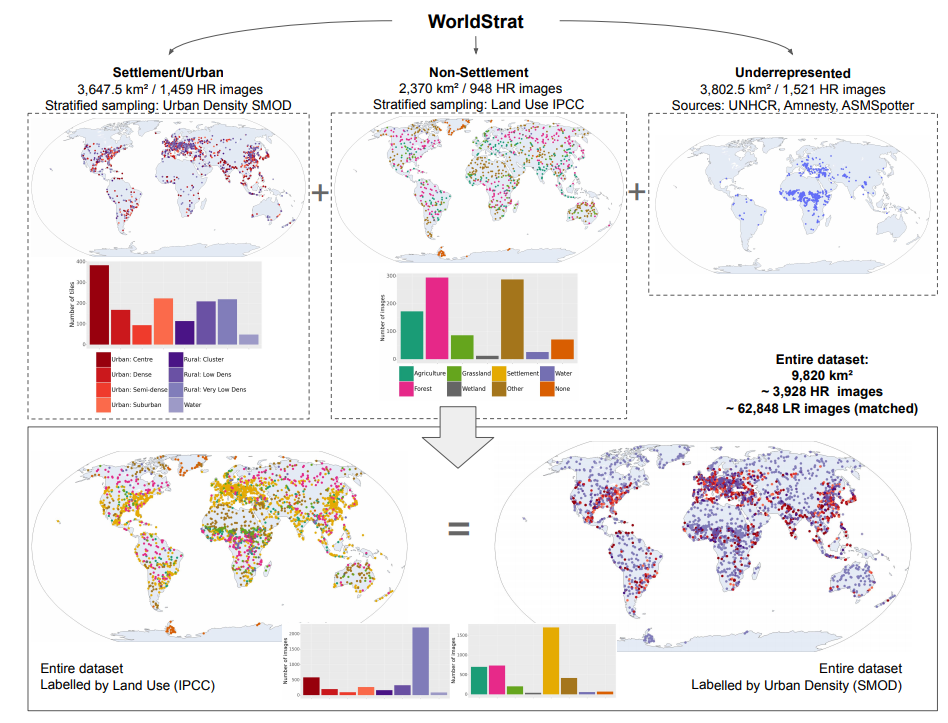
\includegraphics[width=1\linewidth]{images/csaybar_fig07.png}
    \begin{justify}
        \textit{Nota.} Resumen de la construcción y clases del conjunto de datos WorldStrat. Obtenido de \textcite{cornebise2022open}
    \end{justify}                    
    \label{fig:worldstrat}
\end{figure}

\subsection{Sen2Venus Dataset}
SEN2VENμS es un conjunto de datos extenso diseñado específicamente para mejorar la resolución espacial de ocho bandas de Sentinel-2 a 5 metros. Consiste en parches de reflectancia de superficie sin nubes capturados por Sentinel-2 L2A a 10 metros y 20 metros, junto con parches de referencia correspondientes adquiridos por el satélite VENμS a una resolución de 5 metros el mismo día. El conjunto de datos cubre 29 ubicaciones diferentes en todo el mundo, abarcando un total de 132,955 parches, cada uno con un tamaño de 256 × 256 píxeles (Figura \ref{fig:sen2venus}).

\begin{figure}[H] 
    \caption{\doublespacing \\ \textit{Mapa de cobertura de Sentinel-2 en Theia (naranja), sitios VENμS disponibles (verde) y 29 sitios seleccionados (rojo) para el conjunto de datos.}} 
    \centering
    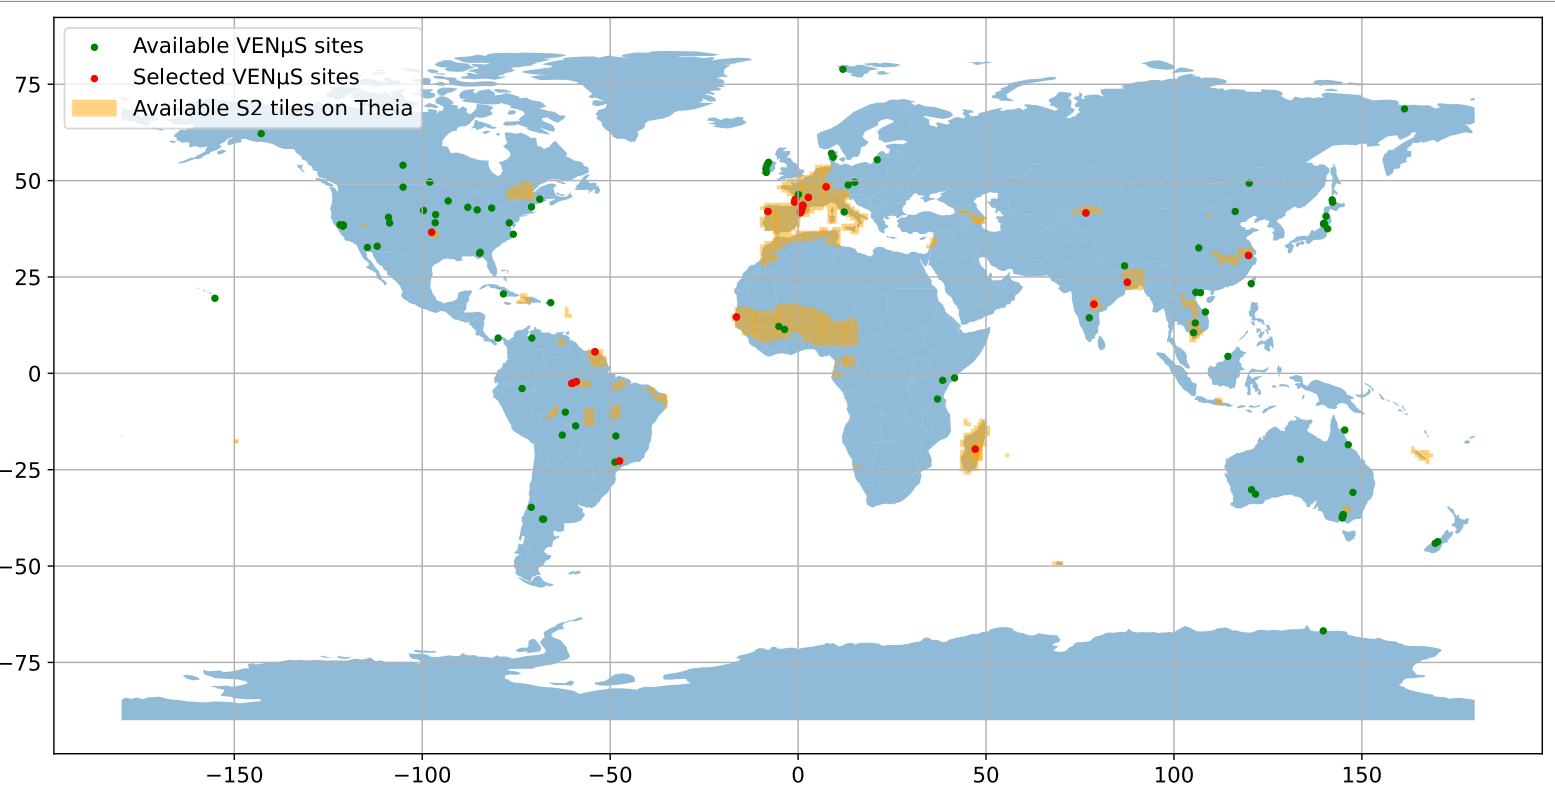
\includegraphics[width=1\linewidth]{images/csaybar_fig06.png}
    \begin{justify}
        \textit{Nota.} Mapa de cobertura de Sentinel-2 en Theia (naranja), sitios VENμS disponibles (verde) y 29 sitios seleccionados (rojo) para el conjunto de datos. Obtenido de \textcite{michel2022sen2venmus}
    \end{justify}                    
    \label{fig:sen2venus}
\end{figure}

\subsection{Degraded Sentinel-2 Dataset}
Los conjuntos de datos introducidos anteriormente presentan cualidades y desventajas específicas. Uno de los factores a equilibrar es el tamaño del conjunto de datos en comparación con la calidad y adecuación de los datos. En un extremo, WorldStrat es de muy alta calidad y está estrechamente conectado con el tipo de superresolución que deseamos realizar, mientras que en el otro extremo, el conjunto de datos OpenImages es enorme, pero no tiene conexión con imágenes de teledetección. Para tener imágenes en el dominio espectral de Sentinel-2 y en el ámbito de la teledetección, se ha muestreado una gran cantidad de imágenes Sentinel-2 RGB-NIR en todo el mundo (Figura \ref{fig:sampling_sites}).

Las imágenes tienen, naturalmente, la resolución estándar de Sentinel-2 de 10 metros, que se utiliza como la versión HR. La versión LR del par de imágenes se crea aplicando un núcleo de degradación a la imagen de HR, produciendo un par de imágenes LR-HR RGB-NIR con resoluciones espaciales de 40 y 10 metros respectivamente, para un factor de superresolución de 4. De esta forma, se crean más de 250,000 pares de imágenes, proporcionando un conjunto de datos que no presenta problemas con desajustes espectrales, temporales o geométricos y que ya se encuentra en el dominio de Sentinel-2. La única desventaja es que la frecuencia de información cambia, ya que la escala de los objetos en el suelo es significativamente diferente. Aun así, este conjunto de datos es muy útil para entrenar redes desde cero o para un ajuste más rudo después de ser entrenado en conjuntos de datos de imágenes naturales. Después de eso, los conjuntos de datos NAIP y WorldStrat pueden proporcionar el toque final.

\begin{figure}[H] 
    \caption{\doublespacing \\ \textit{Áreas de muestreo (gris) y ubicaciones (rojo) de imágenes Sentinel-2 sin nubes.}} 
    \centering
    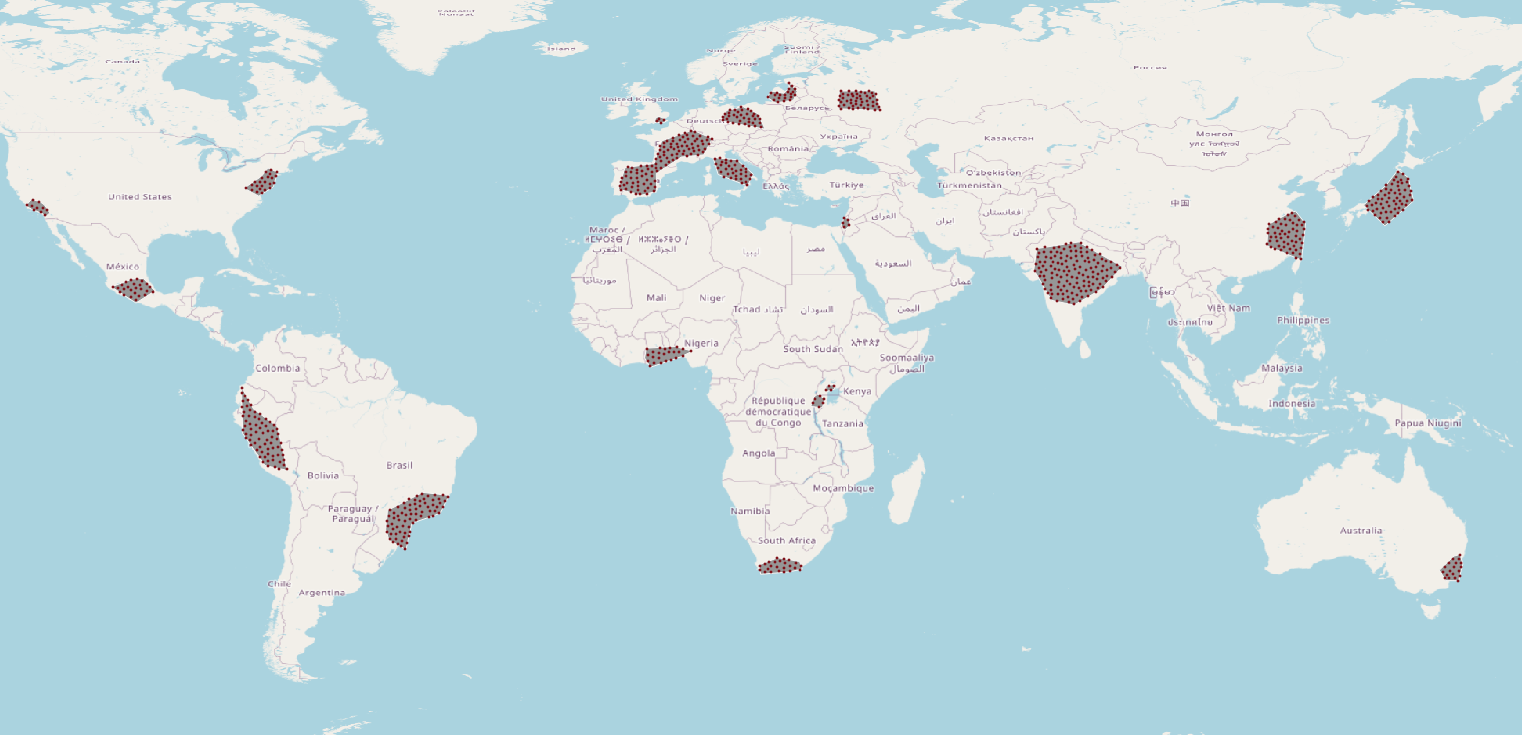
\includegraphics[width=1\linewidth]{images/sampling_locations.png}
    \begin{justify}
        \textit{Nota.} Áreas de muestreo (gris) y ubicaciones (rojo) de imágenes Sentinel-2 sin nubes.
    \end{justify}                    
    \label{fig:sampling_sites}
\end{figure}

\begin{figure}[H] 
    \caption{\doublespacing \\ \textit{Ejemplo del conjunto de datos degradado de Sentinel-2.}} 
    \centering
    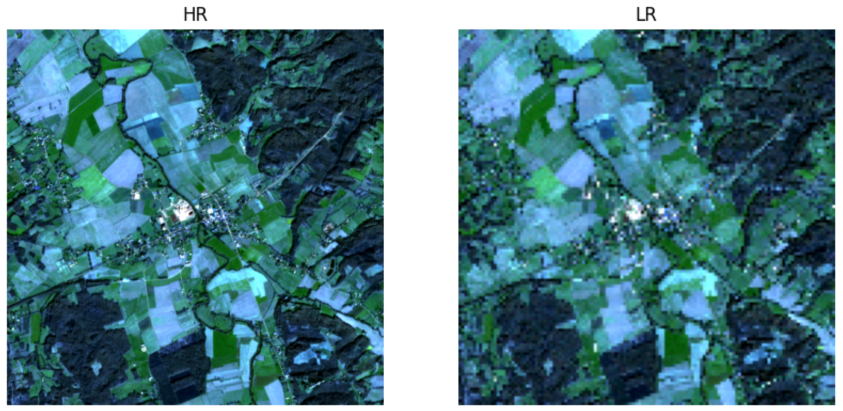
\includegraphics[width=1\linewidth]{images/sen2_degr.png}
    \begin{justify}
        \textit{Nota.} Ejemplo del conjunto de datos degradado de Sentinel-2 (HR: 10m, LR: 40m). Si bien las propiedades espectrales son inconfundiblemente parecidas a Sentinel-2, la frecuencia de la información espacial es claramente diferente de los conjuntos de datos de 2.5m-10m.
    \end{justify}                    
    \label{fig:sen2_degraded}
\end{figure}

\section{Armonización de Datos}

\subsection{Resolución espacial efectiva y PSF}

Comprender la relación entre la resolución espacial efectiva y la Función de Dispersión de Punto (PSF, por sus siglas en inglés) es esencial para una interpretación precisa de los modelos de superresolución. En nuestro estudio, el término resolución espacial efectiva se emplea para denotar la resolución espacial medida por la distancia de muestreo en el suelo, en lugar de simplemente caracterizarla por el tamaño del píxel. El concepto de distancia de muestreo en el suelo (GSD, por sus siglas en inglés) se refiere a la capacidad del sistema para delinear pequeños objetos dentro de una imagen. El GSD está influenciado por varios factores, incluyendo el diseño del sensor, el ángulo de visión y las técnicas de preprocesamiento de imágenes. Estos factores pueden modelarse de manera efectiva utilizando una o múltiples PSF (Figura \ref{fig:psf}).

\begin{figure}[H] 
    \caption{\doublespacing \\ \textit{Representación gráfica que ilustra la Función de Dispersión de Punto (PSF) de un sistema de imagen óptica.}} 
    \centering
    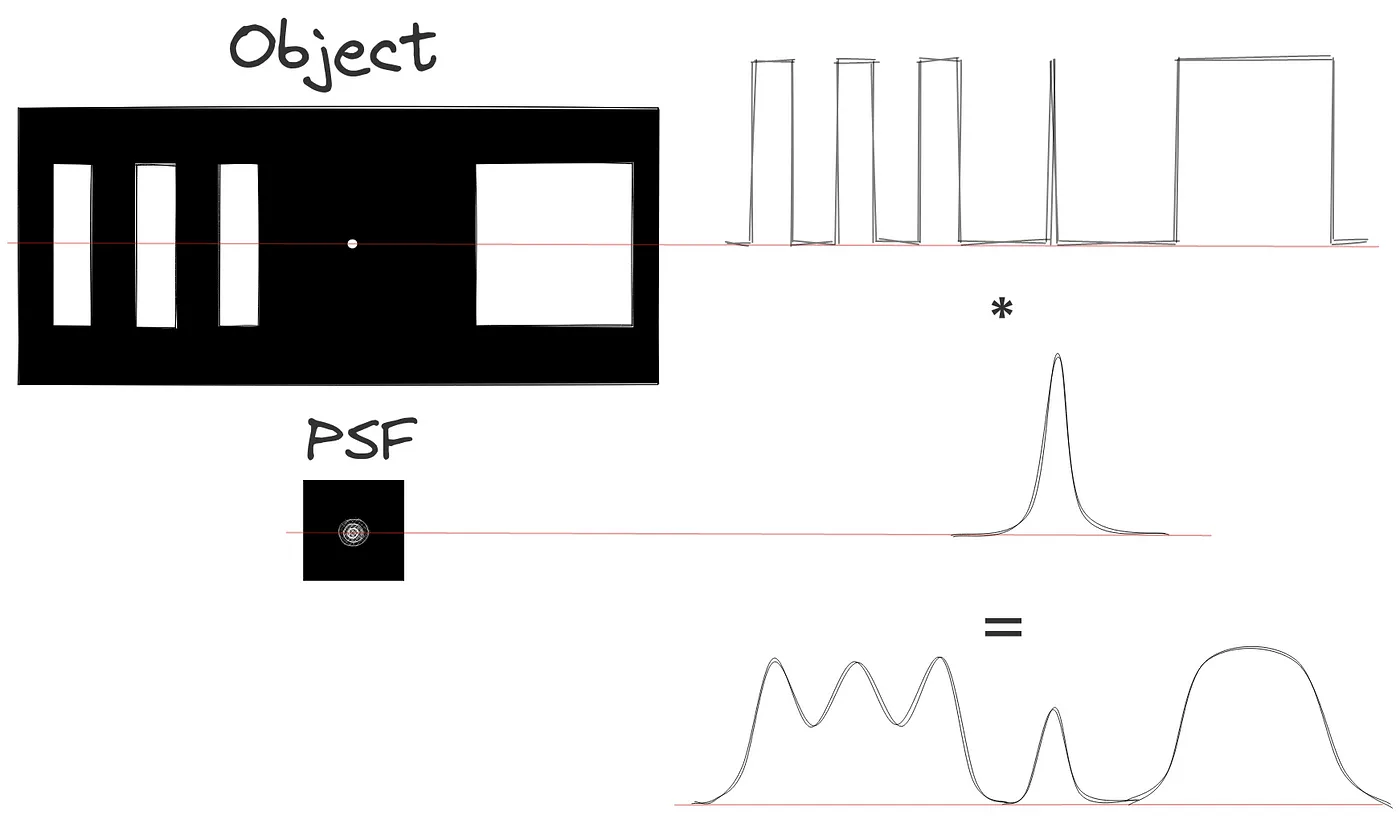
\includegraphics[width=1\linewidth]{images/csaybar_new_fig01.png}
    \begin{justify}
        \textit{Nota.} Representación gráfica que ilustra la Función de Dispersión de Punto (PSF) de un sistema de imagen óptica. La extensión de la dispersión impacta directamente en la resolución espacial, lo que significa que cuando es mayor, la capacidad para distinguir objetos individuales disminuye.
    \end{justify}                    
    \label{fig:psf}
\end{figure}

La PSF caracteriza la respuesta de un sistema de imágenes a una fuente puntual o un solo píxel. Describe cómo la energía de un objeto se dispersa en la imagen, afectando la nitidez, la resolución y la precisión espacial de la imagen. A través del modelado de los atributos de la PSF, es posible emular las funcionalidades de sistemas de teledetección de baja resolución (LR) utilizando contrapartes de alta resolución (HR).

\subsection{Corregistro Espacial}

En el ámbito de la superresolución, el corregistro espacial sirve como una medida de preprocesamiento esencial para mitigar disparidades entre sensores de alta resolución (HR) y baja resolución (LR). En escenarios prácticos, incluso desalineaciones marginales pueden influir considerablemente en la precisión de las métricas resultantes. En consecuencia, garantizar un corregistro espacial meticuloso se vuelve indispensable para obtener métricas de superresolución confiables y esclarecedoras.

Los algoritmos de corregistro espacial generalmente abarcan tres etapas principales. La primera etapa es la detección de puntos clave, que busca identificar puntos prominentes dentro de una imagen. La siguiente etapa implica la detección de puntos coincidentes entre las imágenes de HR y LR. Finalmente, los errores de desalineación se calculan a través de un modelo polinomial ajustado a estos puntos coincidentes. En los últimos años, se ha presentado una gran variedad de algoritmos para la alineación automática de imágenes. Por ejemplo, el conjunto de datos SEN2VENμS utilizó el algoritmo de coincidencia SIFT \autocite{michel2022sen2venmus}, mientras que MuRA-T comparó los resultados de alineación de los algoritmos Fast+VGG y SuperPoint+SuperGlue \autocite{deshmukh2023aligned}.

\begin{figure}[H]
    \caption{\doublespacing \\ \textit{Puntos coincidentes obtenidos al aplicar el algoritmo SuperPoint + SuperGlue a un par de imágenes.}} 
    \centering
    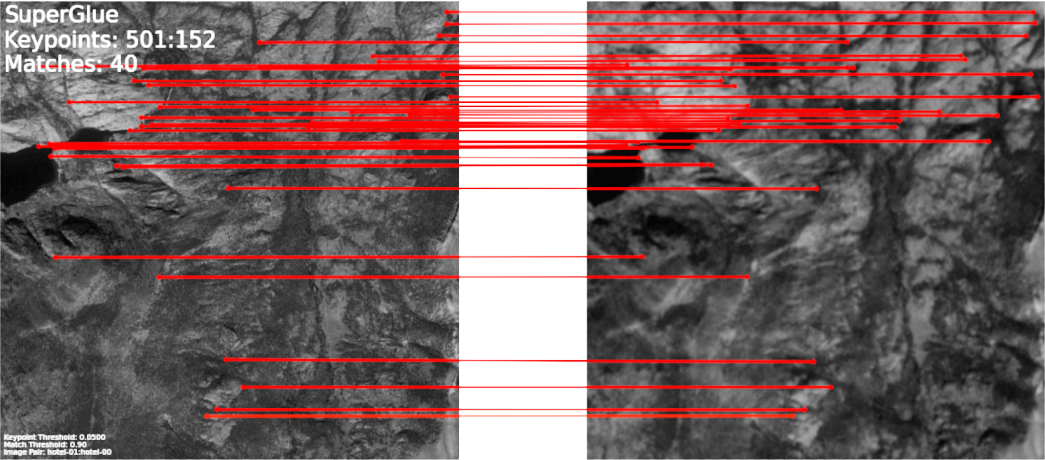
\includegraphics[width=1\linewidth]{images/csaybar_fig01.png}
    \begin{justify}
        \textit{Nota.} Puntos coincidentes obtenidos al aplicar el algoritmo SuperPoint + SuperGlue a un par de imágenes, donde la imagen de baja resolución (LR) es de Sentinel-2 y la imagen de alta resolución (HR) es de NAIP.
    \end{justify}                    
    \label{fig:coregistration}
\end{figure}

\subsection{Calibración e Armonización entre Instrumentos}

Incluso cuando dos sensores de teledetección adquieren datos el mismo día, aún pueden existir variaciones significativas en sus valores. Estas variaciones pueden atribuirse a varios factores, que incluyen:

\begin{itemize}
    \item \textbf{Características del sensor}: Cada sensor tiene su propia función de respuesta espectral única, lo que puede resultar en variaciones en los valores de reflectancia, incluso cuando las condiciones atmosféricas y el ángulo de visión son los mismos.

    \item \textbf{Condiciones atmosféricas}: La atmósfera puede experimentar cambios significativos en pocos minutos o segundos. Estas variaciones pueden afectar la calidad y precisión de los datos capturados por los sensores de teledetección. La dispersión atmosférica, por ejemplo, puede introducir variaciones en las señales del sensor, lo que lleva a diferencias en los valores de reflectancia.

    \item \textbf{Geometría de visión}: La diferencia entre el ángulo desde el cual los sensores observan la superficie de la Tierra también puede llevar a variaciones en los valores de reflectancia.

    \item \textbf{Calibración y preprocesamiento}: Cada sensor pasa por su propio proceso de calibración para convertir las mediciones en bruto en valores de reflectancia significativos. Estas variaciones deben ser cuidadosamente tenidas en cuenta y abordadas durante la comparación LR-HR.
    
\end{itemize}

Para minimizar las posibles variaciones en la reflectancia entre los pares LR-HR, se propone un componente adicional para mejorar el modelo de degradación clásico.

\begin{equation}
    I_{LR} = \gamma[\delta(I_{HR}, \eta)] + \epsilon
\end{equation}

Donde $I_{LR}$ es la imagen LR, $I_{HR}$ es la imagen HR, $\eta$ es un parámetro del modelo de degradación $\delta$, $\epsilon$ representa el ruido, y $\gamma$ el modelo de armonización.